\documentclass[tikz,border=6pt]{standalone}
\usepackage{pgfplots}
\pgfplotsset{compat=1.18}
\usepgfplotslibrary{colormaps}
\usetikzlibrary{arrows, arrows.meta, calc}
\usetikzlibrary{decorations.markings}


\usepackage{amssymb,amsmath,mathtools}

\usepackage[T1]{fontenc}
\usepackage[utf8]{inputenc}
\usepackage{newpxtext,newpxmath}
\usepackage{sectsty}

\renewcommand{\Re}{\operatorname{\mathrm{Re}}}
\renewcommand{\Im}{\operatorname{\mathrm{Im}}}


\begin{document}
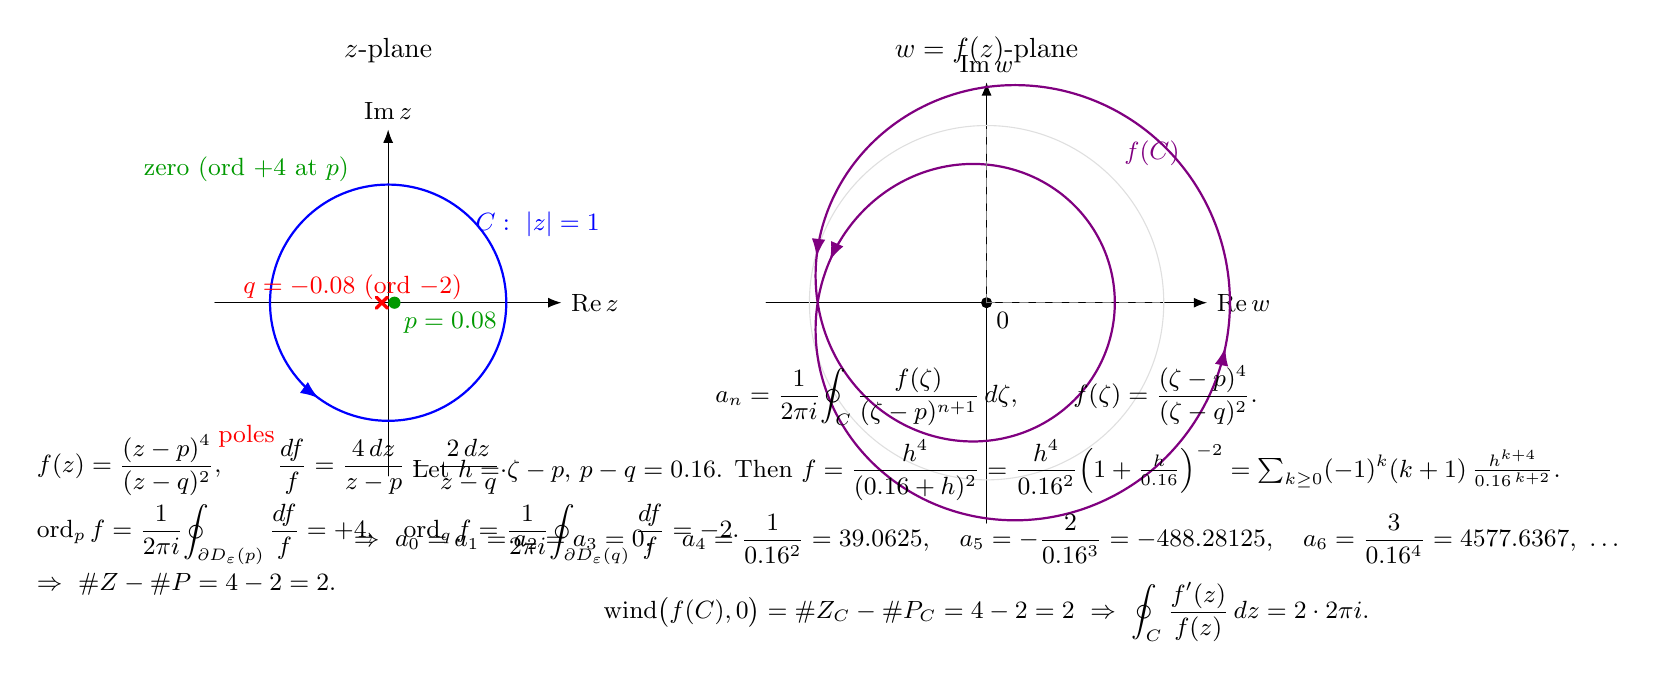
\begin{tikzpicture}[>=Latex, line cap=round, line join=round, font=\small]
	
	%========================
	% Left: z-plane
	%========================
	\begin{scope}[shift={(0,0)}]
		\node[font=\normalsize] at (0,3.2) {$z$-plane};
		% axes
		\draw[->] (-2.2,0)--(2.2,0) node[right] {$\Re z$};
		\draw[->] (0,-2.2)--(0,2.2) node[above] {$\Im z$};
		
		% unit circle C (positively oriented) -- drawn with radius 1.5 for visibility
		\draw[blue,thick,postaction={decorate},
		decoration={markings, mark=at position 0.65 with {\arrow{>}}}]
		(0,0) circle (1.5);
		\node[blue] at (1.9,1.0) {$C:\ |z|=1$};
		
		% zero at p (order +4) and pole at q (order -2), kept very close to 0 so f(C) stays near-circle
		\fill[green!60!black] (0.08,0) circle(2.2pt) node[below right] {$p=0.08$};
		\node[green!60!black] at (-1.8,1.7) {zero (ord $+4$ at $p$)};
		\draw[red,very thick] (-0.08,0) ++(-0.07,-0.07) -- ++(0.14,0.14);
		\draw[red,very thick] (-0.08,0) ++(-0.07,0.07)  -- ++(0.14,-0.14);
		\node[red] at (-0.45,0.2) {$q=-0.08$ (ord $-2$)};
		\node[red] at (-1.8,-1.7) {poles};
		
		% function label + orders via the winding / log-derivative form
		\node[align=left] at (0,-2.7) {$\displaystyle
			f(z)=\frac{(z-p)^4}{(z-q)^2},\qquad
			\frac{df}{f}=\frac{4\,dz}{z-p}-\frac{2\,dz}{z-q}.$\\[2pt]
			$\displaystyle \operatorname{ord}_{p} f=\frac{1}{2\pi i}\!\oint_{\partial D_\varepsilon(p)}\frac{df}{f}=+4,\quad
			\operatorname{ord}_{q} f=\frac{1}{2\pi i}\!\oint_{\partial D_\varepsilon(q)}\frac{df}{f}=-2.$\\[2pt]
			$\Rightarrow\ \#Z-\#P=4-2=2.$};
	\end{scope}
	
	%========================
	% Right: w-plane = f(z)-plane
	%========================
	\begin{scope}[shift={(7.6,0)}]
		\node[font=\normalsize] at (0,3.2) {$w=f(z)$-plane};
		% axes
		\draw[->] (-2.8,0)--(2.8,0) node[right] {$\Re w$};
		\draw[->] (0,-2.8)--(0,2.8) node[above] {$\Im w$};
		
		% origin and a faint reference circle (shows the image stays near-scale)
		\fill (0,0) circle(2pt) node[below right] {$0$};
		\draw[gray!25] (0,0) circle (2.25); % ≈ (1.5^4)/(1.5^2) = 1.5^2
		
		% image curve f(C): z = x+iy = 1.5 e^{it} -> w = (z-p)^4/(z-q)^2
		% Choose p=+0.08, q=-0.08 (small and symmetric so f(C) stays close to a circle)
		% Set x=1.5 cos t, y=1.5 sin t.
		% u = x - p = x - 0.08, v = y                            (so z-p = u + i v).
		% a = x - q = x + 0.08, b = y                            (so z-q = a + i b).
		% Numerator: (u+iv)^4 = Nre + i Nim with
		%   Nre = u^4 - 6 u^2 v^2 + v^4
		%   Nim = 4 u^3 v - 4 u v^3
		% Denominator: (a+ib)^2 = Dre + i Dim with
		%   Dre = a^2 - b^2
		%   Dim = 2 a b
		% Then w = N / D with
		%   Re w = (Nre*Dre + Nim*Dim) / (Dre^2 + Dim^2)
		%   Im w = (Nim*Dre - Nre*Dim) / (Dre^2 + Dim^2)
		\draw[violet,thick,
		postaction={decorate},
		decoration={markings,
			mark=at position 0.18 with {\arrow{>}},
			mark=at position 0.48 with {\arrow{>}},
			mark=at position 0.78 with {\arrow{>}}}]
		plot[domain=0:6.283, samples=750]
		({
			% Re w
			(
			% Nre*Dre
			( (1.5*cos(\x r)-0.08)^(4)
			- 6*(1.5*cos(\x r)-0.08)^(2)*(1.5*sin(\x r))^(2)
			+ (1.5*sin(\x r))^(4) )
			*
			( (1.5*cos(\x r)+0.08)^(2) - (1.5*sin(\x r))^(2) )
			+
			% Nim*Dim
			( 4*(1.5*cos(\x r)-0.08)^(3)*(1.5*sin(\x r))
			- 4*(1.5*cos(\x r)-0.08)*(1.5*sin(\x r))^(3) )
			*
			( 2*(1.5*cos(\x r)+0.08)*(1.5*sin(\x r)) )
			)
			/
			(
			% Dre^2 + Dim^2
			( (1.5*cos(\x r)+0.08)^(2) - (1.5*sin(\x r))^(2) )^(2)
			+
			( 2*(1.5*cos(\x r)+0.08)*(1.5*sin(\x r)) )^(2)
			)
		},
		{
			% Im w
			(
			% Nim*Dre
			( 4*(1.5*cos(\x r)-0.08)^(3)*(1.5*sin(\x r))
			- 4*(1.5*cos(\x r)-0.08)*(1.5*sin(\x r))^(3) )
			*
			( (1.5*cos(\x r)+0.08)^(2) - (1.5*sin(\x r))^(2) )
			-
			% Nre*Dim
			( (1.5*cos(\x r)-0.08)^(4)
			- 6*(1.5*cos(\x r)-0.08)^(2)*(1.5*sin(\x r))^(2)
			+ (1.5*sin(\x r))^(4) )
			*
			( 2*(1.5*cos(\x r)+0.08)*(1.5*sin(\x r)) )
			)
			/
			(
			( (1.5*cos(\x r)+0.08)^(2) - (1.5*sin(\x r))^(2) )^(2)
			+
			( 2*(1.5*cos(\x r)+0.08)*(1.5*sin(\x r)) )^(2)
			)
		});
		\node[violet] at (2.1,1.9) {$f(C)$};
		
		% dashed rays to visualize winding (here: +2)
		\draw[gray,dashed] (0,0) -- (2.2,0);
		\draw[gray,dashed] (0,0) -- (0,2.2);
		
		% annotation: Taylor coefficients at z_0=p via Cauchy integrals (explicit numbers)
		\node[align=center] at (0,-2.55)
		{$\displaystyle
			a_n=\frac{1}{2\pi i}\!\oint_C \frac{f(\zeta)}{(\zeta-p)^{n+1}}\,d\zeta,
			\qquad f(\zeta)=\frac{(\zeta-p)^4}{(\zeta-q)^2}.$\\[4pt]
			Let $h=\zeta-p$, $p-q=0.16$. Then
			$f=\dfrac{h^4}{(0.16+h)^2}
			=\dfrac{h^4}{0.16^2}\Big(1+\frac{h}{0.16}\Big)^{-2}
			=\sum_{k\ge0}(-1)^k(k+1)\,\frac{h^{k+4}}{0.16^{\,k+2}}.$\\[4pt]
			$\Rightarrow\ a_0=a_1=a_2=a_3=0,\quad
			a_4=\dfrac{1}{0.16^2}=39.0625,\quad
			a_5=-\dfrac{2}{0.16^3}=-488.28125,\quad
			a_6=\dfrac{3}{0.16^4}=4577.6367,\ \ldots$\\[6pt]
			$\mathrm{wind}\big(f(C),0\big)=\#Z_C-\#P_C=4-2=2
			\ \Rightarrow\
			\displaystyle \oint_C \frac{f'(z)}{f(z)}\,dz=2\cdot 2\pi i.$};
	\end{scope}
	
\end{tikzpicture}
\end{document}